% !TEX TS-program = pdflatex
% !TEX encoding = UTF-8 Unicode

% This is a simple template for a LaTeX document using the "article" class.
% See "book", "report", "letter" for other types of document.

\documentclass{llncs}
              
\usepackage[utf8]{inputenc} % set input encoding (not needed with XeLaTeX)

%%% Examples of Article customizations
% These packages are optional, depending whether you want the features they provide.
% See the LaTeX Companion or other references for full information.

%%% PAGE DIMENSIONS
\usepackage{geometry} % to change the page dimensions
\geometry{a4paper} % or letterpaper (US) or a5paper or....
% \geometry{margin=2in} % for example, change the margins to 2 inches all round
% \geometry{landscape} % set up the page for landscape
%   read geometry.pdf for detailed page layout information

\usepackage{graphicx} % support the \includegraphics command and options

% \usepackage[parfill]{parskip} % Activate to begin paragraphs with an empty line rather than an indent

%%% PACKAGES
\usepackage{booktabs} % for much better looking tables
\usepackage{array} % for better arrays (eg matrices) in maths
\usepackage{paralist} % very flexible & customisable lists (eg. enumerate/itemize, etc.)
%\usepackage{proof}
\usepackage{verbatim} % adds environment for commenting out blocks of text & for better verbatim
\usepackage{subfig} % make it possible to include more than one captioned figure/table in a single float
\usepackage{xcolor}
%\usepackage{amsmath}
%\usepackage{amssymb}
%\usepackage{amsthm}
\usepackage{algpseudocode}
\usepackage{enumerate}
\usepackage{bussproofs}
\usepackage{algorithm}
\usepackage{tikz}
\usetikzlibrary{shapes.geometric, arrows}
\usepackage{flowchart}
\usepackage{hyperref}
\usepackage{wrapfig}
%\usepackage{subcaption}
\tikzstyle{startstop} = [rectangle, rounded corners, minimum width=3cm, minimum height=1cm,text centered, draw=black, fill=red!30]
\tikzstyle{process} = [rectangle, minimum width=3cm, minimum height=1cm, text centered, draw=black, fill=orange!30]
\tikzstyle{decision} = [diamond, minimum width=3cm, minimum height=1cm, text centered, draw=black, fill=green!30]
\tikzstyle{arrow} = [thick,->,>=stealth]


% These packages are all incorporated in the memoir class to one degree or another...

%%% HEADERS & FOOTERS
\usepackage{fancyhdr} % This should be set AFTER setting up the page geometry
\pagestyle{fancy} % options: empty , plain , fancy
\renewcommand{\headrulewidth}{0pt} % customise the layout...
\lhead{}\chead{}\rhead{}
\lfoot{}\cfoot{\thepage}\rfoot{}

%%% SECTION TITLE APPEARANCE
\usepackage{sectsty}
\allsectionsfont{\sffamily\mdseries\upshape} % (See the fntguide.pdf for font help)
% (This matches ConTeXt defaults)

%%% END Article customizations


\definecolor{darkblue}{rgb}{0,0,0.6}
\definecolor{darkgreen}{rgb}{0,0.6,0}
\usepackage{listings}
\lstnewenvironment{smtlib}
{\lstset{language=Lisp,
    basicstyle=\ttfamily,
    commentstyle=\color{darkgreen},
    stringstyle=\color{red},
    keywordstyle=\color{darkblue}\bfseries,
    showstringspaces=false,
    morekeywords={set-logic,declare-fun,assert,declare-const,or,and},
    escapeinside={@}{@}}}
{}


\newcommand{\implies}{\Rightarrow}
\newcommand{\Int}{\mathcal{Z}}
\newcommand{\Core}{\mathcal{C}}
\newcommand{\Clause}{C}

\newcommand{\forward}{\mathit{forward}}
\newcommand{\papercomment}[1]{}

\newcommand{\mod}{\ \mbox{mod}\ }
\newcommand{\constraint}{sc}
\newcommand{\overmul}[2]{\Omega^*(#1,#2)}
\newcommand{\overmuls}[2]{\Omega_s^*(#1,#2)}
\newcommand{\overadd}[2]{\Omega^+(#1,#2)}
\newcommand{\binop}{\mathit{binop}}
\newcommand{\conflictlevel}[1]{\mathit{level}(#1)}
\newcommand{\assignment}[2]{\langle #1, #2 \rangle}
\newcommand{\parity}[1]{\mathit{parity}(#1)}
\newcommand{\polysat}{\textsc{PolySAT}}
\newcommand{\stp}{\textsc{STP}}
\newcommand{\cvcfive}{\textsc{cvc5}}
\newcommand{\boolector}{\textsc{Boolector}}
\newcommand{\bitwuzla}{\textsc{Bitwuzla}}
\newcommand{\uclid}{\textsc{uclid}}
\newcommand{\mathsat}{\textsc{MathSAT}}
\newcommand{\wombit}{\textsc{Wombit}}
\newcommand{\yicestwo}{\textsc{Yices2}}
\newcommand{\zthree}{\textsc{Z3}}

\newcommand{\sat}{\mathsf{Sat}}
\newcommand{\unsat}{\mathsf{Unsat}}

% object-level equality
\newcommand{\eql}{\simeq}
\newcommand{\neql}{\not\eql}

\newcommand{\concat}{\mathbin{+\!\!\!+}}
\newcommand{\bvshl}{\mathbin{<\!\!\!<}}
\newcommand{\bvshr}{\mathbin{>\!\!\!>}}
\newcommand{\bvand}{\mathbin{\&}}
\newcommand{\bvor}{\mathbin{|}}
\newcommand{\bvnot}{{\sim}}

%\newcommand{\rem}{\operatorname{rem}}
\newcommand{\rem}[2]{#1 \perc #2}
\newcommand{\bit}[2]{#1[#2]}
\newcommand{\divop}[2]{#1 \mathbin{/} #2}
\newcommand{\inv}[1]{\operatorname{inv}(#1)}
\newcommand{\modop}{\operatorname{mod}}
\newcommand{\bor}[2]{#1 \bvor #2}
\newcommand{\bnot}[1]{{\bvnot}#1}
\newcommand{\extract}[3]{#1[#2{:}#3]}   % \extract{x}{hi}{lo}       x[hi:lo]
\newcommand{\msb}[2]{#1[{:}#2]}         % \msb{x}{lo}               x[:lo]
\newcommand{\lsb}[2]{#1[#2{:}]}         % \lsb{x}{hi}               x[hi:]
\newcommand{\rshiftop}[2]{#1 \bvshr #2}
\newcommand{\lshiftop}[2]{#1 \bvshl #2}

\newcommand\rulename[1]{\textsc{#1}}
\newcommand{\UnsatRule}{\rulename{Unsat}\xspace}
\newcommand{\SatRule}{\rulename{Sat}\xspace}
\newcommand{\BooleanDecideRule}{\rulename{BoolDec}\xspace}
\newcommand{\BooleanPropagateRule}{\rulename{BoolProp}\xspace}
\newcommand{\BooleanConflictRule}{\rulename{BoolConf}\xspace}
\newcommand{\TheoryPropagateRule}{\rulename{TheoryProp}\xspace}
\newcommand{\TheoryConflictRule}{\rulename{TheoryConf}\xspace}
\newcommand{\ValueDecideRule}{\rulename{ValueDec}\xspace}
\newcommand{\ValuePropagateRule}{\rulename{ValueProp}\xspace}
\newcommand{\EvaluateRule}{\rulename{Evaluate}\xspace}
\newcommand{\EvaluateTopRule}{\rulename{Evaluate}$_\top$\xspace}
\newcommand{\EvaluateBottomRule}{\rulename{Evaluate}$_\bot$\xspace}
\newcommand{\ViableConflictRule}{\rulename{ViableConf}\xspace}
\newcommand{\ValueConflictRule}{\rulename{ValueConf}\xspace}
\newcommand{\BooleanResolutionRule}{\rulename{BoolRes}\xspace}
\newcommand{\ValueResolutionRule}{\rulename{ValueRes}\xspace}
\newcommand{\LemmaRule}{\rulename{Lemma}\xspace}
\newcommand{\LearnRule}{\rulename{Learn}\xspace}
\newcommand{\BackjumpRule}{\rulename{Backjump}\xspace}
\newcommand{\SaturateRule}{\rulename{Saturate}\xspace}
\newcommand{\SkipRule}{\rulename{Skip}\xspace}
\newcommand{\ReplayRule}{\rulename{Replay}\xspace}
\newcommand\myeq{\mkern1.5mu{=}\mkern1.5mu}

\newcommand{\Eval}[2]{\mathit{Eval}(#1;#2)}
\newcommand{\EvalN}{\mathit{Eval}}
\newcommand{\search}[2]{#1 \mid #2}
\newcommand{\conflict}[4]{#1 \mid #2 \mid #3 \mid #4}
\newcommand{\Viable}{\mathit{Viable}}
\newcommand{\onenorm}[1]{|\!|#1|\!|_1}

% See also https://tex.stackexchange.com/a/326251 if we need a resizable version (using \DeclarePairedDelimiterX)
\newcommand{\interval}[2]{\ensuremath{\mathopen[{#1};{#2}\mathclose[}}
% interval closed-closed
\newcommand{\intervalcc}[2]{\ensuremath{\mathopen[{#1};{#2}\mathclose]}}

\newcommand{\Zmod}[1]{\mathbb{Z}/{#1}\mathbb{Z}}
\newcommand{\idiv}{\;\mathrm{div}\;}
\newcommand{\eval}[1]{\beta(#1)}

%%% The "real" document content comes below...

\title{Arithmetic Solving in Z3}
\author{Nikolaj Bj\o{}rner\and
  Lev Nachmanson}
\institute{Microsoft}

\newcommand{\NB}[1]{{\color{orange}NB: #1}}
\newcommand{\LEV}[1]{{\color{red}LN: #1}}


\begin{document}
\maketitle

\begin{abstract}
  The theory of arithmetic is integral to many uses of SMT solvers.
  Z3 has implemented native solvers for arithmetic reasoning since its first release.
  We present a full re-implementation of Z3's original
  arithmetic solver. It is based on substantial experiences from user feedback, engineering and experimentation.
  While providing a comprehensive overview of the main components
  we emphasize selected new insights we arrived at while developing and testing the solver.
\end{abstract}

\section{Introduction}

The theory of arithmetic
is among the most prolific theories used in SMT solvers. It is used across a wide set of
applications, and they have a wide range of demands.
Supporting efficient theory solvers for arithmetic requires balancing feature support,
ranging from linear, difference logic, to linear real, linear integer, non-linear polynomial arithmetic
and in cases transcendental functions such as exponentiation.
The aim of this paper is to provide a high-level, yet self-contained, overview of internal ingredients of the arithmetic solver.
It seeks to explain tool users what to expect of solving methodologies when using Z3 for arithmetic.
We assume familiarity of basics of SMT solving using CDCL(T), e.g.,~\cite{z3internals}.
While make an effort to cover all features for completeness,
we devote attention to highlight a selection that to our knowledge are unique for arithmetic solvers.
These highlights include
(1) how the new solver patches linear real programming solutions to find solutions to integer variables,
(2) heuristics that are new in how the solver finds Gomory cuts, and
(3) the solver's integration of Gr{\"o}bner basis computation for solving non-linear constraints.
User pain points around SMT have to our experience centered dominantly
around quantifiers and non-linear arithmetic. A complete (for non-linear reals) solver that integrates
with other theories and quantifier reasoning becomes relevant.
To evaluate the contribution of each feature we use benchmarks drawn
from SMTLIB benchmark sets~\cite{SMTLIB2} and benchmarks supplied by a user, 
Certora~\cite{bench-submission}.

In overview, the arithmetic solver uses a waterfall model for solving arithmetic constraints.
It is illustrated with additional details in Figure~\ref{fig:organization}.


\begin{itemize}
  \item First, it establishes feasibility with respect to linear inequalities. Variables are solved over the rationals; Section~\ref{sec:lp}.
  \item Second, it establishes feasibility with respect to mixed integer linear constraints; 
        Integer variables are considered solved if they are assigned integer values while satisfying linear inequalities; Section~\ref{sec:ip}. 
  \item Finally, it establishes feasibility with respect to non-linear polynomial constraints; Section~\ref{sec:nla}.
\end{itemize}


\begin{figure}[htbp]
  \centering
  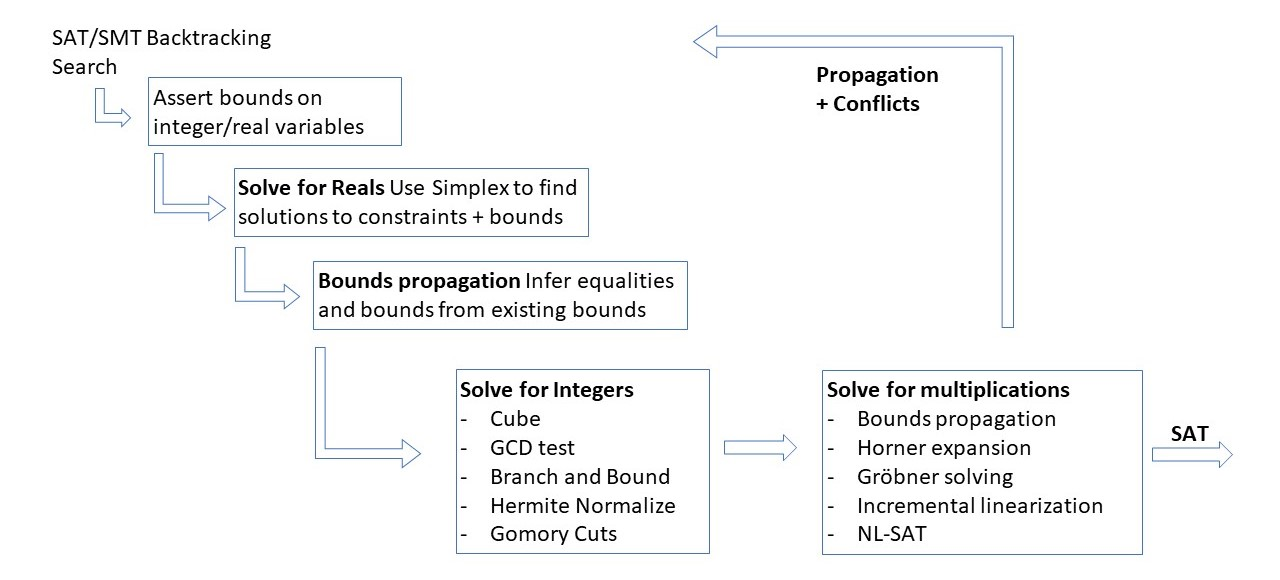
\includegraphics[width=0.99\textwidth]{figures/Arithmetic.jpg}
  \caption{Overview of Z3's Arithmetic Theory Solver }
  \label{fig:organization}
\end{figure}

The rest of the paper elaborates on the components of the solver. For completeness, we
go through all relevant pieces. We highlight parts that to our knowledge are novel.

%In the following we will ``unpeal'' the onion comprising of the ingredients in
%each of the three phases and also how they are integrated.
%The overall behavior of the arithmetic solver is a combination of many parts;
%an advance in each part contributes to the overall advance of the solver.
%For benchmarks from applications we observe that there is no single component that
%is single-handedly responsible for ``cracking the code''.

\papercomment{
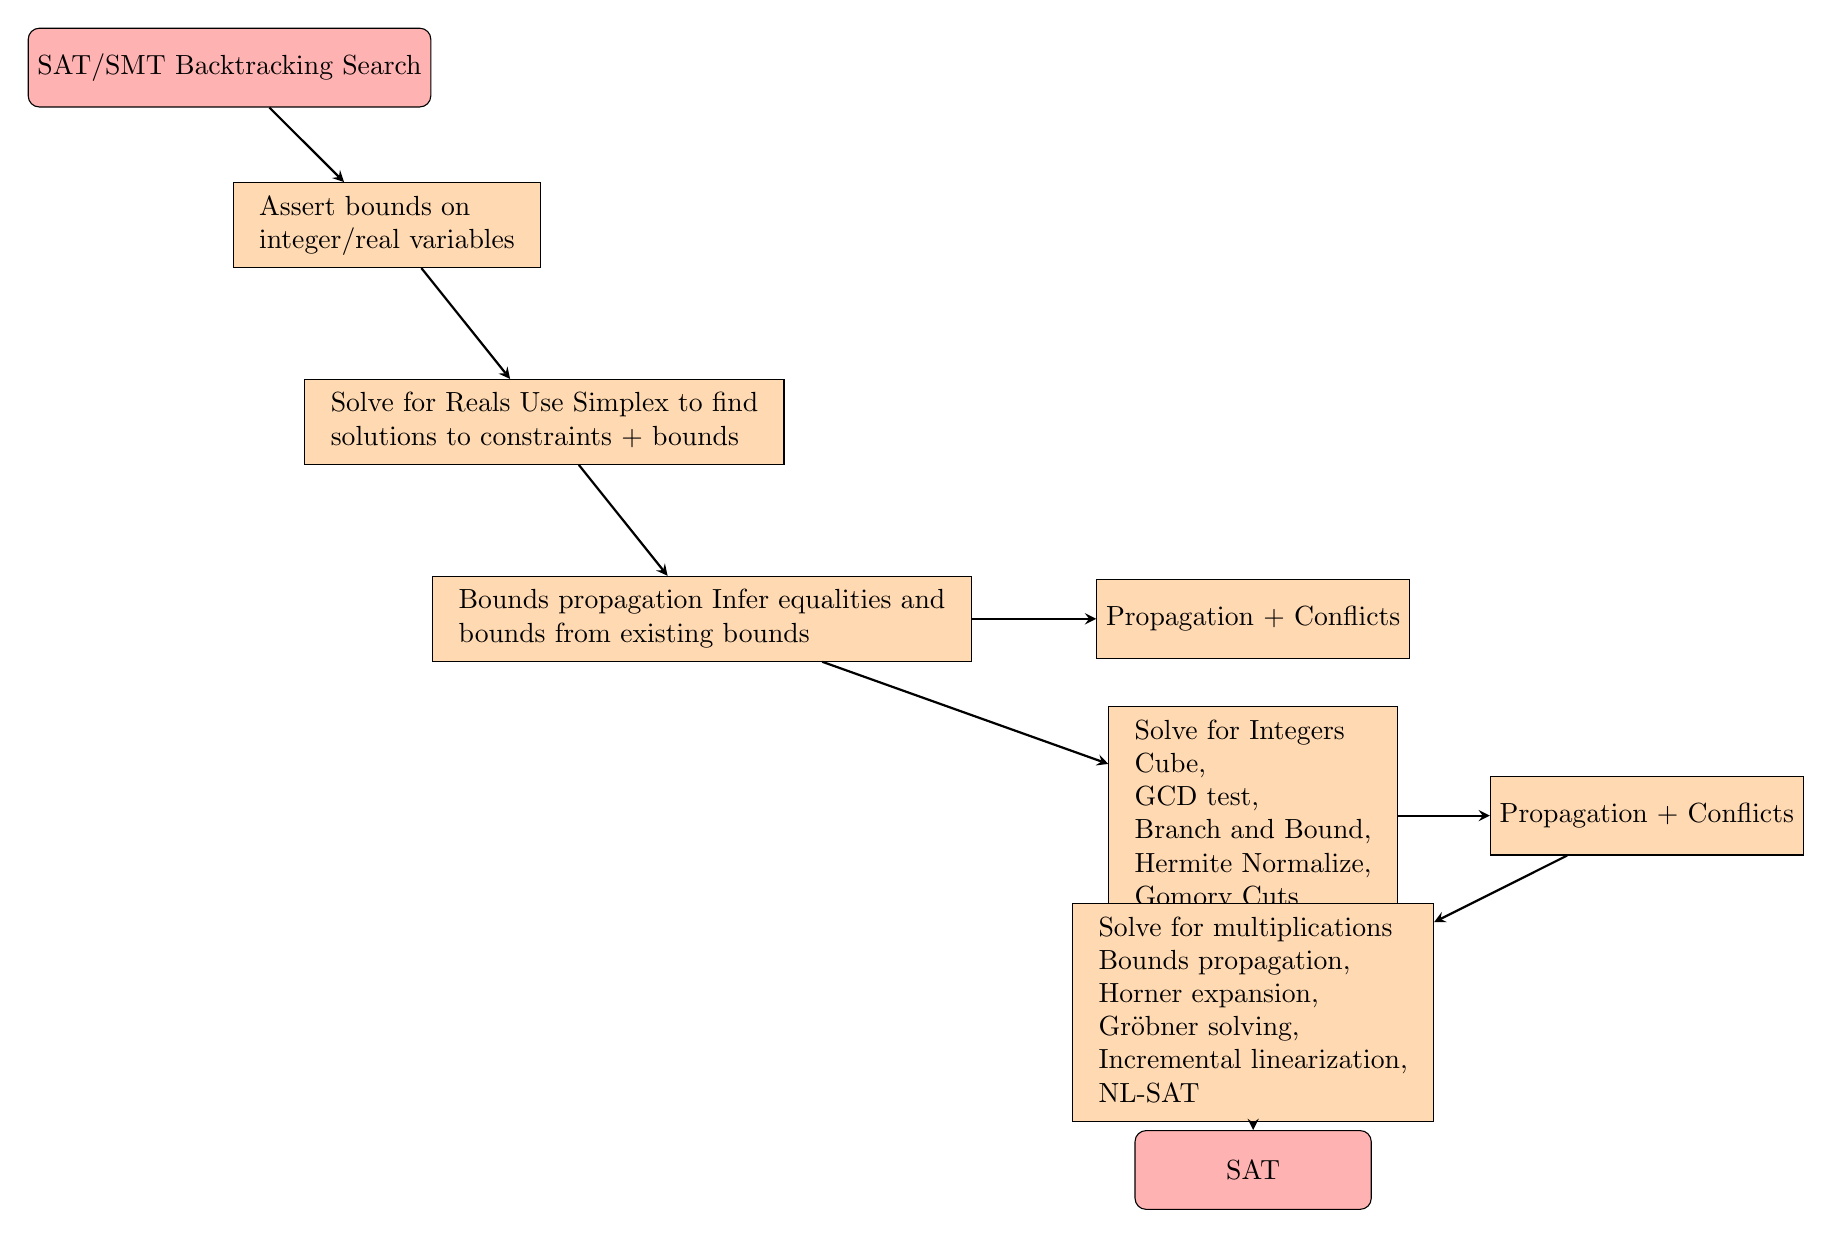
\begin{tikzpicture}[node distance=2cm]
    \node (start) [startstop] {SAT/SMT Backtracking Search};
    \node (pro1) [process, below of=start, right of=start] {\begin{tabular}{l}Assert bounds on \\ integer/real variables\end{tabular}};
    \node (pro2) [process, below of=pro1, right of=pro1, yshift=-0.5cm] {\begin{tabular}{l}Solve for Reals Use Simplex to find \\ solutions to constraints + bounds\end{tabular}};
    \node (pro3) [process, below of=pro2, right of=pro2, yshift=-0.5cm] {\begin{tabular}{l} Bounds propagation Infer equalities and \\ bounds from existing bounds\end{tabular}};
    \node (pro4) [process, right of=pro3, right of=pro3, xshift=3cm] {Propagation + Conflicts};
    \node (pro5) [process, below of=pro4, yshift=-0.5cm] {\begin{tabular}{l}Solve for Integers\\
        Cube, \\
        GCD test, \\
        Branch and Bound, \\
        Hermite Normalize, \\
        Gomory Cuts
    \end{tabular}};
    \node (pro7) [process, right of=pro5, xshift=3cm] {Propagation + Conflicts};
    \node (pro8) [process, below of=pro5, yshift=-0.5cm] {\begin{tabular}{l}Solve for multiplications\\
        Bounds propagation, \\
        Horner expansion, \\
        Gr{\"o}bner solving, \\
        Incremental linearization, \\
        NL-SAT
    \end{tabular}};
    \node (end) [startstop, below of=pro8] {SAT};
    \draw [arrow] (start) -- (pro1);
    \draw [arrow] (pro1) -- (pro2);
    \draw [arrow] (pro2) -- (pro3);
    \draw [arrow] (pro3) -- (pro4);
    \draw [arrow] (pro3) -- (pro5);
    \draw [arrow] (pro5) -- (pro7);
    \draw [arrow] (pro7) -- (pro8);
    \draw [arrow] (pro8) -- (end);
\end{tikzpicture}
}


\papercomment{
  \subsection{Notes}

\begin{itemize}
  \item For a set of equations in form $x \pm y$ find fixed variables based on the variable values. Consider a graph formed by edges $(x,y)$, break it into connected components, and use pivoting to transform each component into a star.

\end{itemize}
}

\section{Design Goals and Implementation Choices}

The SMT formalism for arithmetic in many cases subsumes formalisms used by mixed integer, MIP, solvers.
However, there are several fundamental differences between the workloads we have tuned the arithmetic
solver for compared to workloads seen by MIP solvers.
Z3 uses infinite precision ``big-num'' numeral representations, in contrast to using floating points.
The drawback is that the arithmetic solver is impractical on linear programming optimization problems,
but the engine avoids having to compensate for rounding errors and numerical instability.
The solver uses a sparse matrix representation
for the Dual Simplex tableau.
We also created a version that uses an LRU decomposition and floating
point numbers but found that extending this version with efficient backtracking was not practical
compared to the straight-forward sparse matrix format.
Finally, the solver remains integrated within a CDCL engine that favors an eager case split strategy
leaving it to conflict analysis to block infeasible branches. This contrasts mainstream MIP designs
that favor a search tree of relatively few branches where the engine performs significant analysis before case splits.

%The arithmetic solver reduces operations such as integer modulus, remainder, and division into equations.
%It eagerly compiles bounds axioms of the form $x \geq 3 \implies x \geq 2$ for atomic formulas $x \geq 3, x\geq 2$.


\section{Linear Real Arithmetic}
\label{sec:lp}
The solver first determines whether arithmetic constraints are feasibility over the reals.
It also attempts to propagate equalities eagerly for shared variables and infer stronger bounds of variables.

\subsection{Linear Solving}

Based on~\cite{DutertreM06} the solver for real linear inequalities uses a dual simplex solver.
It partitions the variables into \emph{basic} and \emph{non-basic} variables, and maintains
a global set of equalities of the form $x_{bi} + \sum_j a_{ij}x_j = 0$,
where $i$ refers to the $i$'th row, $x_{bi}$ is basic and $x_j$ range over non-basic variables.
It also maintains an evaluation
$\beta$, such that $\eval{x_{bi}} + \sum_j a_{ij}\eval{x_j}= 0$ for each row $i$.
Each variable $x_j$ is assigned lower and upper bounds during search.
The solver then checks whether $lo_j \leq \eval{x_j} \leq hi_j$, for bounds
$lo_j, hi_j$ that are dynamically added and removed by Boolean decisions $x_j \leq hi_j$, $x_j \geq lo_j$.
If the bounds are violated, it updates the evaluation and pivots if necessary.
We recall the approach using an example.

\begin{example}

For the following formula
\[
 y \geq 0 \land (x + y \leq 2 \lor x + 2y \geq 6) \land (x + y \geq 2 \lor x + 2y > 4)
\]
the solver introduces auxiliary variables $s_1, s_2$ and represents the formula as
\[
  x + y - s_1 = 0, x + 2y - s_2 = 0, \
  x \geq 0, (s_1 \leq 2 \vee s_2 \geq 6), (s_1 \geq 2 \vee s_2 > 4)
\]

Only bounds (e.g., $s_1 \leq 2$) are asserted during search.
The slack variables $s_1, s_2$ are initially basic (dependent) and $x, y$ are non-basic.
In dual Simplex tableaux, values of a non-basic variable
$x_j$ can be chosen between $lo_j$ and $hi_j$.
The value of a basic variable is a function of non-basic variable values.
Pivoting swaps basic and non-basic variables and moves basic variables within their bounds to bounds violations.
For example, assume we start with a set of initial values
$x = y = s_1 = s_2 = 0$
and bounds $x \geq 0, s_1 \leq 2, s_1 \geq 2$. 
Then $s_1$ has to be 2 and it is made non-basic. 
Instead, $y$ becomes basic:
$
{y} + x - s_1 = 0, \ {s_2} + x - 2s_1 = 0.
$
The new tableau updates the assignment of variables to
$x = 0, s_1 = 2, s_2 = 4, y = 2$. The resulting assignment
is a model for the original formula.

\end{example}

\subsection{Finding equal variables - cheaply}
It is useful to have the arithmetic solver propagate implied equalities when arithmetic is used in combination with other theories, or even when
it solves non-linear arithmetic constraints. Equality propagation is disabled for pure arithmetic theories, such as {\tt QF\_LIA, QF\_LRA}~\cite{SMTLIB2}.
Z3 originally used a method based on storing \emph{offset} equalities in a hash table.
An offset equality is of the form $x_i = y + k$, where $k$ is a numeric constant.
Offset equalities are extracted from rows that contain $x_i$ as a basic variable, and contains
only one other non-fixed variable $y$, while other variables are fixed and their lower
(upper) bounds add up to $k$. It turns out that computing $k$ is
expensive when the tableau contains large numeric constants. Hash table operations
contribute with additional overhead. It turns out that neither the offset hash-table, nor computing $k$,
is really necessary. We describe our new method, using an example.
We first described the method for avoiding to compute offsets in~\cite{DBLP:conf/sbmf/BjornerN20}.
The description there relies on building a tree data-structure for connecting variables and fails to leverage that the dual simplex tableau can be
used directly.


\begin{example}

From equalities $x + 1 = y, y - 1 = z$ infer that $x = z$. Based on the tableau form, the solver is presented with the original equality atoms via slack variables
\[
    s_1 = x + u - y, s_2 = y - u - z, 1 \leq u \leq 1
    \]	
The tableau can be solved by setting $x = 0, y = 0, z = 0, s_1 = 1, s_2 = -1, u = 1$.
The slack variables are bounded when the equalities are asserted
\[
    s_1 = x + u - y, s_2 = y - u - z, 1 \leq u \leq 1, 0 \leq s_1 \leq 0, 0 \leq s_2 \leq 0
    \]
The original solution is no longer valid, the values for $s_1, s_2$ are out of bounds.
Pivoting re-establishes feasibility using a different solution, for example
\[
    x = z - u - s_1, y = z - u - s_2, 1 \leq u \leq 1, 0 \leq s_1 \leq 0, 0 \leq s_2 \leq 0
    \]
with assignment $z = 0, x = y = -1$. The variables $x$ and $y$ have the same value,
but must they be equal under all assignments? We can establish this directly by subtracting the
right-hand sides $z - u - s_1$ and $z - u - s_2$ from another and by factoring in the constant bounds to obtain
the result $0$. But subtraction is generally expensive if there are many bounded constants in the rows.
Such arithmetical operations are not required to infer that $x = y$.

\end{example}

Z3 uses the following conditions to infer an equality between variables $x, y$ having the same values in the current assignment:
\begin{itemize}
    \item $x$ is basic, and the tableau has row $x - y + \alpha = 0$,
    \item $x, y$ are connected through a non-basic variable $z$ in a pair of the tableau rows in one of the following forms
	(1) $x - z + \alpha = 0, y - z + \alpha' = 0$, (2) $x + z + \alpha = 0, y + z + \alpha' = 0$, 	
\end{itemize}
where $\alpha, \alpha'$ are linear combinations of fixed variables.

We experimented with generalizing the connection between equal variables to
allow non-unit coefficients on $z$, but it did not result in measurable improvements.


\subsection{Bounds Propagation}
\label{sec:bounds-propagation}
It is not uncommon that SMT formulas contain different bounds for the same variable, such as one atom $x \geq 2$ and another atom $x \geq 3$.
When the atom $x \geq 3$ is assigned to true, the solver can directly propagate $x \geq 3$. Bounds can also be inferred indirectly.
With a row $x - 2y = 0$ and bound $y \geq 1$, it follows that $x \geq 2$. To implement direct bounds propagation, the solver
maintains an index that maps each variable to the set of bounds atoms where it occurs. To implement indirect bounds propagation,
the solver queries updated rows for whether they imply bounds that are stronger than the currently asserted bounds. If so, these
stronger bounds are used by the index for direct bounds propagation.

\section{Integer Linear Arithmetic}
\label{sec:ip}

The mixed integer linear solver consists of several layers that first attempt to \emph{patch} integer variables
form solutions over reals to solutions over integers. Then, if patching fails to correct all integer variables,
it checks for integer infeasibility by checking light-weight Diophantine feasibility criteria and then resort to variants of
Gomory Cuts and Branch and Bound.


\subsection{Patching}


In a feasible tableau we can assume that all non-basic variables are at their bounds
and therefore if they have integer sort they are assigned integer values.
Only the basic variables could be assigned non-integer values.
Patching seeks changing values of non-basic values in order to assign integer values to basic variables.
A related method, that diversifies values of variables using \emph{freedom} intervals was
described in~\cite{MouraB08}, but we found it does not preserve integral assignments.

Thus, we patch rows with basic variables $x_b \not\in\Int$.
We use a process that seeks a $\delta$, such that $|\delta|$ is minimal
and the row with $x_b$ is of the form $x_b + \alpha y + \alpha'x' = 0$,
where $\alpha \not\in \Int$,
such that the update $\eval{y} := \eval{y} + \delta$ is within the bounds of $y$,
$x_b$ is assigned an integer value and such that $x_b$ becomes integer without 
breaking any bounds in the tableau.
%We describe details of the patching method in Appendix~\ref{app:ip-patching}.


\begin{example}
  Suppose we are given a tableau of the form
  $
 y - \frac{1}{2} x = 0, \ 
 z - \frac{1}{3} x  = 0
$
where $y, z$ are basic variables and $x$ has bounds $[3,10]$, $y$ has bounds $[-3,4]$, $z$ has bounds $[-5,12]$.
The variable $x$ is initially assigned at the bound $\eval{x} = 3$. Then $\eval{y} = \frac{3}{2}$ and
$\eval{z} = 1$. But neither $y$ nor $z$ is close to their bounds. We can move $x$ to $8$
without violating the bound for $y$ because of $y - \frac{1}{2} x = 0$.
Thus, the freedom interval for $x$ is the range $[3,8]$ and within this range there is a solution,
$x = 6$, where $y, z$ are integers and within their bounds.
\end{example}



\subsection{Cubes}
An important factor in solving more satisfiable integer arithmetic instances is
a method by Bromberger and Weidenbach~\cite{BrombergerW16,BrombergerW17}.
It allows detecting feasible inequalities over integer variables 
by solving a stronger linear system.
Their method relies on the following property: The inequalities $Ax \leq b$
are integer feasible, for matrix $A$ and vectors $x, b$, if
$Ax \leq b - \frac{1}{2}\onenorm{A}$ has a solution over the reals.
We use the 1-norm $\onenorm{A}$ of a matrix
as a column vector, such that each entry $i$ is the sum of the absolute
values of the elements in the corresponding row $A_i$.

\begin{example}
Suppose we have $3x + y \leq 9 \wedge - 3y \leq -2$ and wish to find an integer solution. 
By solving $3x + y \leq 9 - \frac{1}{2}(3 + 1) = 7, -3y \leq -2 - \frac{1}{2}3 = -3.5$ we find
a model where $y = \frac{7}{6}, x = 0$. After rounding $y$ to $1$ and maintaining $x$ at $0$ we obtain an
integer solution to the original inequalities.
\end{example}

Z3 includes a twist relative to~\cite{BrombergerW17} that allows to avoid strengthening on selected inequalities~\cite{Vampire17Theorem}.
First, we note that \emph{difference} inequalities of the form $x - y \leq k$, where $x, y$ are integer variables
and $k$ is an integer offset need not be strengthened: they have a solution over reals if and only if they have a solution over integers.
For octagon constraints $\pm x \pm y \leq k$,
there is a boundary condition: they need only require strengthening if $x, y$ are assigned at mid-points
between integral solutions. For example, if $\eval{x} = \frac{1}{2}$ and $\eval{y} = \frac{3}{2}$, for $x + y \leq 2$.


\subsection{GCD consistency}\label{sec:gcd-consistency}
A basic test for integer infeasibility is by enforcing divisibility constraints.
\begin{example}
  Assume we are given a row $5/6x + 3/6y + z + 5/6u = 0$, where $x, y$ are fixed at $2 \leq x \leq 2$, $-1 \leq u \leq -1$, and $z$ is the base variable.
  Then it follows that $5 + 3(y + 2z) = 0$ which has no solution over the integers:
  The greatest common divisor of coefficients to the non-fixed variables ($3$) does not divide the constant offset from the fixed variables ($5$).
\end{example}
The basic test is extended as follows. For each row $a x + b y + c = 0$, where
\begin{itemize}
  \item $a, b, c$ and $x, y$ are vectors of integer constants and variables, respectively.
  \item the coefficients in $a$ are all the same and smaller than the coefficients in $b$
  \item the variables $x$ are bounded
\end{itemize}
Let $l := a\cdot lb(x), u := a \cdot ub(x)$.
That is, the lower and upper bounds for $a\cdot x$ based on the bounds for $x$.
If $\lfloor \frac{u}{\gcd(b,c)} \rfloor > \lceil  \frac{l}{\gcd(b,c)} \rceil$, then
there is no solution for $x$ within the bounds for $x$.



\subsection{Branching}
Similar to traditional MIP branch-and-bound methods, 
the solver creates somewhat eagerly case splits on bounds 
of integer variables if the dual simplex solver fails to assign them integer values. For example, Simplex may assign an integer variable $x$, the value $\frac{1}{2}$, in which case z3 creates a literal $x \leq 0$ that triggers two branches
$x \leq 0$ and $\neg(x \leq 0) \equiv x \geq 1$.


\subsection{Cuts}\label{sec:cuts}
The arithmetic solver produces Gomory cuts from rows where the basic variables are non-integers after
the non-basic variables have been pushed to the bounds. Z3 implements Chv{\'a}tal-Goromy cuts described in~\cite{DutertreM06}.
It also implements algorithms from~\cite{DilligDA09,ChristH15}
to generate cuts after the linear systems have been transformed into Hermitian matrices.
It is a long-standing and timely challenge~\cite{DBLP:conf/nips/BalcanPSV22} to harness the effectiveness of selecting cuts.
While the solver takes~\cite{DutertreM06} as starting point, it incorporates a few heuristics and enhancements.

Recall that a row $\sum_{j=0}^{k} a_j\cdot x_j + x_b = 0$ 
from the tableau is called a Gomory row, and is eligible for Gomory cut, if $x_b$ is a basic variable and $x_j$ are non-basic variables,
$x_b$ is an integral variable, but $\eval{x_b}$ is not integral, and for each $x_j$ we have $\eval{x_j} = lo_j$ or $\eval{x_j} = hi_j$,
and the bounds are not strict. 

We use a relaxed definition of Gomory rows. For a non-basic integral variable $x_j$ we allow for value $\eval{x_j}$ to be not at a bound when $\eval{x_j}$, and $a_j$ are both integers: Let us call such $x_j$ \emph{row integral}.
%We provide further justification for
%this relaxed definition in Appendix~\ref{app:row-integral}.


To select a cut variable, our main heuristic sorts all Gomory rows from the tableau by the distance of $\eval{x_b}$ from the nearest integer, that is $\min \{ {\eval{x_b}-\lfloor \eval{x_b} \rfloor, \lceil \eval{x_b} \rceil - \eval{x_b}} \}$, and pick a few of them having the minimal distance to produce the cuts. We break the ties by preferring the variables that are used in more terms.
Heuristics used previously relied on distances to bounds.

We also look for the case when $x_b$ is at an extremum. For example, if for all $x_j$ we have $\eval{x_j} = lo_j$,
and $a_j > 0$ then $x_b$ is at the maximum, and we deduce $x_b \leq \lfloor \eval{x_b} \rfloor$.
The explanations of the Gomory term do not include constraints on $x_j$ for $j \in A$ from the relaxed definition,
but in case of an extremum these constraints should be added.

% NSB: does not make sense: if $\eval{x_b} = -\eval{\sum_{j=0}^{k} a_j\cdot x_j}$, then $\eval{x_b}$ will also have to be integral.
%Another consideration is the case of an empty Gomory term:
%it happens when $\sum_{j=0}^{k} a_j\cdot x_j$ is always integral. We report a conflict in this situation.

Cuts are consequences of the current bounds. By default the solver adds new rows to the Dual Simplex tableau corresponding to cuts,
but makes an exception when the new rows include large numerals.
In analogy the solver avoids bounds propagation, Section~\ref{sec:bounds-propagation},
when computation of bounds relies on big-num arithmetic.
Similarly, cuts that involve large coefficients are first added to a temporary scope where the tableau is checked for feasibility.
The cuts are only re-added within the main scope if the temporary tableau is infeasible.


\section{Non-Linear Arithmetic}
\label{sec:nla}

Similar to solving for integer feasibility, the arithmetic solver
solves constraints over polynomials using a waterfall model for non-linear
constraints.
At the basis it maintains, for every monomial 
term $x \cdot x \cdot y$, a definition
$m = x \cdot x \cdot y$, where $m$ is a variable
that represents the monomial $x \cdot x \cdot y$.
The module for non-linear arithmetic then collects the monomial
definitions that are violated by the current evaluation,
that is $\eval{m} \neq \eval{x} \cdot \eval{x} \cdot \eval{y}$. It  attempts to 
establish a valuation $\beta'$ where $\beta'(m) = \beta'(x) \cdot \beta'(x) \cdot \beta'(y)$, 
or derive a consequence that no such evaluation exists.



\subsection{Patch Monomials}

A \emph{patch} for a variable $x$ is \emph{admissible} if the update $\eval{x} := v$
does not break any integer linear constraints and $x$ does not occur in monomial
equations that are not already false under $\beta$.

\begin{itemize}
\item Set $\eval{m} := \eval{x} \cdot \eval{x} \cdot \eval{y}$ and check if the patch of $m$ is admissible.
\item Try to set $\eval{y} := \eval{m} / (\eval{x} \cdot \eval{x})$, provided $\beta{x}$ is not 0,
  and check that the patch for $x$ is admissible.
\item When $\eval{m} = r^2$ for a rational and $m := x \cdot x$ try patching $x$ by setting $\eval{x} := \pm r$.
\end{itemize}


\subsection{Bounds propagation}
A relatively inexpensive step is to propagate and check bounds based 
on non-linear constraints. For example, for $y \geq 3$, then $m = x\cdot x\cdot y \geq 3$,
if furthermore $x \leq -2$, we have the strengthened bound $m \geq 12$.
Bounds propagation can also flow from bounds on $m$ to bounds on the 
variables that make up the monomial, such that when $m \geq 8, 1 \leq y \leq 2, x \leq 0$, 
then we learn the stronger bound $x \leq -2$ on $x$. It uses an interval arithmetic abstraction,
that understands bounds propagation over squares. Thus, if $-2 \leq x \leq 2$, then $0 \leq x^2 \leq 4$
instead of $-4 \leq x^2 \leq 4$.

The solver also performs Horner expansions of polynomials to derive stronger bounds.
For example, if $x \geq 2, y \geq -1, z \geq 2$, then $y + z \geq 1$ 
and therefore $x\cdot (y + z) \geq 2$, but we would not be
able to deduce this fact if combining bounds individually for $x\cdot y$ 
and $x \cdot z$ because no bounds can be inferred for $x \cdot y$ in isolation.
The solver therefore attempts different re-distribution of multiplication
in an effort to find stronger bounds.


\subsection{Adding bounds}
Non-linear bounds propagation only triggers if all variables are either bounded from above or below or occur with an even power.
The solver includes a pass where it adds a bound case split $x \geq 0$ to variables $x$ where $lo_x = -\infty, hi_x = +\infty$.
The added case split may help trigger bounds propagation, such as detecting conflicts on $xy > 0, xz > 0, y > 0 > z$.


\subsection{Gr{\"o}bner reduction}

Z3 uses a best effort Gr\"obner basis reduction to find inconsistencies, cheaply, 
and propagate consequences. While Gr{\"o}bner basis heuristics are not new to Z3,
they have evolved and to our knowledge the integration is unique among SMT solvers.
Recall that reduced Gr{\"o}bner basis for a set of polynomial equations $p_1 = 0, \ldots, p_k = 0$
is a set $q_1 = 0, \ldots, q_m = 0$, such that every $p_i$ is a linear sum of $q_j$'s,
and the leading monomials of every pair $q_i, q_j$, $i \neq j$, have no common factors.
Since Z3 uses completion as a heuristic to make partial inferences, it does not seek to compute
a basis.
The Gr\"obner module performs a set of partial completion steps, preferring
to eliminate variables that can be isolated, and expanding a bounded number of super-position
steps (reductions by S-polynomials).

Z3 first adds equations $m = x_1\ldots x_k$ for monomial definitions that are violated.
It then traverses the transitive cone of influence of Simplex rows that contain one of the added variables
from monomial definitions. It only considers rows where the basic variable is bounded.
Rows where the basic variable is unbounded are skipped
because the basic variable can be solved for over the reals.
Fixed variables are replaced by constants, and the bounds constraints that fixes the variables
are recorded as dependencies with the added equation. Thus, the equations handled by the
Gr{\"o}bner basis reduction are of the form $\langle p_i: xy + 3z + 3 = 0, d_i: \{3 \leq u \leq 3\} \rangle$, where $p_i$
is a polynomial and $d_i$ is a set of dependencies corresponding to fixed variables that were replaced
by constants in $p_i$. In the example, we replaced $u$ by $3$ and the definition $\langle m = xy, \emptyset\rangle$ resolved $m$ by $xy$.
Dependencies are accumulated when two polynomials are resolved to infer a new derived equality.
Generally, when $\langle xy + p_1 = 0, d_1\rangle, \langle xz + p_2 = 0, d_2 \rangle$ are two polynomial equations,
then $\langle zp_1 - yp_2 = 0, d_1 \cup d_2\rangle$ can be derived accumulating the premises $d_1, d_2$.

Finally, equations are pre-solved if they are linear and can be split
into two groups, one containing a single variable that has a
lower (upper) bound, the other with more than two variables
with upper (lower) bounds. This avoids losing bounds information
during completion.

After (partial) completion, the derived equations are post-processed:
\begin{description}

\item[Constant propagation]
For equalities of the form $x = 0$ or $ax + b = 0$. If the current assignment to $x$ does not
satisfy the equation, then the equality is propagated as a lemma.

\item[Linear propagation]
As a generalization of constant propagation, if the completion contains linear equations that
evaluate to false under the current assignment, then these linear equations are added to the
Simplex Tableau. Example~\ref{ex:yoav} illustrates a use where this propagation is useful.

\item[Factorization] Identify factors of the
form $x y p \simeq 0$ where $x, y$ are variables an $p$ is linear. We infer 
the clause $x y p \simeq 0 \implies x \simeq 0 \lor y \simeq 0 \lor p \simeq 0$.

\end{description}

\begin{example}[Combining Gr{\"o}bner completion and Linear Solving]
\label{ex:yoav}
We include an example obtained from Yoav Rodeh at Certora.
The instance was not solvable prior to adding simplex propagation.
To solve it, Certora relied on treating multiplication as an uninterpreted function and
including selected axioms for modular arithmetic and multiplication that were instantiated by E-matching.
The distilled example is:

\[
   L \leq x \cdot y \leq U \land 1 \leq x \land m_r \leq U \land x \cdot y \neq m_r
\]
where $L = N \idiv 2, U = 1 + L$, $m_r = (x \cdot (\mathit{ite}(y \geq 0, y, N + y))) \mod N$.
We assume $N$ is even, such as $N = 2^{256}$.
The solver associates a variable $m$ with $x \cdot y$ and $m'$ with $x \cdot y'$ and $y'$ with $\mathit{ite}(y \geq 0, y, N + y)$
and includes the constraints $0 \leq m_r < N, m_q \cdot N + m_r = m'$, where $m_q$ is an integer variable.
The most interesting case is where $y < 0$, so $y' = y + N$. Gr{\"o}bner basis completion
then allows to derive $m_q N + m_r = m' = x(y + N) = xy + xN = m + xN$, which by integer linear arithmetic reasoning (the extended GCD test)
contradicts $m \neq m_r$ because the absolute value of both variables is below $N$.
\end{example}

Our extraction of linear constraints represents a partial integration of linear programming and polynomial arithmetic,
that favors only including linear inequalities over variables and monomials that are already present. Our implementation
does not include any variables for new monomials produced by completion.
In comparison, the approach in~\cite{DBLP:journals/pacmpl/KincaidKZ23} proposes a domain for abstract interpretation that populates a linear
solver with all equations produced by a completion. We have not experimented in depth with extending our approach with a full basis,
or use it as a starting point for finding lemmas based on Positivstellensatz or other extension mechanisms~\cite{DBLP:conf/csl/Tiwari05,DBLP:conf/cade/PlatzerQR09}.





\usetikzlibrary{shapes,arrows}
\usetikzlibrary{positioning}

\tikzstyle{block} = [rectangle, draw, text centered, rounded corners, minimum height=2em]
\tikzstyle{line} = [draw, -latex']

\begin{wrapfigure}{r}{0.4\textwidth} 
  \begin{center}
    \begin{tikzpicture}[node distance = 3em, scale = 0.2]
  \node [circle, draw] (xroot) {$x$};
  \node [circle, below of = xroot, left of= xroot, draw] (xnext) {$x$};
  \node [circle, below of = xnext, left of= xnext, draw] (y1) {$y$};
  \node [circle, below of = xnext, right of = xnext] (yempty) {};
  \node [circle, right of= yempty, draw] (y2) {$y$};
  \node [circle, below of = y1, left of = y1] (t1) {$5$};
  \node [circle, below of = y1, right of = y1] (t2) {$0$};
  \node [circle, right of = t2] (t3) {$1$};
  \node [circle, below of = y2, right of = y2] (t4) {$1$};
  \path [line] (xroot.west) -- (xnext.north);
  \path [line] (xroot.east) -- (y2.north);
  \path [line] (xnext.west) -- (y1.north);
  \path [line] (xnext.east) -- (y2.north);
  \path [line] (y1.west) -- (t1.north);
  \path [line] (y1.east) -- (t2.north);
  \path [line] (y2.west) -- (t3.north);
  \path [line] (y2.east) -- (t4.north);

\end{tikzpicture}

  \end{center}
  \vspace{1pt}
  \caption{PDD representation of $5x^2y + xy + y + x + 1$\label{fig:pdd}}
\end{wrapfigure}
We use an adaptation of ZDD (Zero suppressed decision diagrams~\cite{Minato93,NishinoYMN16}) to represent polynomials.
The representation has the advantage that polynomials are stored in a shared data-structure and operations
over polynomials are memoized. A polynomial over the real is represented as an acyclic graph, where 
nodes are labeled by variables and edges are labeled by coefficients. Figure~\ref{fig:pdd} shows a polynomial stored
in a polynomial decision diagram, PDD.


The root node labeled by $x$ represents the polynomial $x\cdot l + r$, 
where $l$ is the polynomial of the left sub-graph and $r$ the polynomial
of the right sub-graph. The left sub-graph is allowed to be labeled again by $x$, 
but the right sub-graph may only have nodes labeled by variables that are smaller
in a fixed ordering. The fixed ordering used in this example sets $x$ above $y$.
Then the polynomial for the right sub-graph is $y + 1$, and the polynomial with the
left sub-graph is $5xy + (y + 1)$.




\subsection{Incremental linearization}
Following~\cite{CimattiGIRS18} we incrementally linearize monomial definitions that
currently evaluate to false.
For example, we include lemmas of the form $x = 0 \rightarrow m = 0$
and $x = 1 \rightarrow m = y$, for $m = x^2y$.
Incremental linearization proceeds by first applying linearizations that are considered cheap,
such as case splitting on whether variables take values 0, 1, -1, when these boundary conditions
are exhausted, instantiates lemmas based on monotonicity of multiplication and tangents.
It is possible that there are overlapping monomial definitions, such as $m' = x \cdot y$.
Then incremental linearization takes into account that the definition for $m$ can be
\emph{factored} into $m' \cdot x$. It also uses specialized congruence closure reasoning,
recognizing equalities modulo signs, such that when $m = x \cdot y, m' = z \cdot y$ and
$x = -z$ in the current context, then $m \sim -m'$.

% LN, not sure if it is a good place, and 
To find all factorizations of monomial $m = \prod_{i \in A}{x_i} $ as $m = m_0 \cdot m_1$, we choose $a \in A$ and enumerate over all proper subsets $B$ of $A$ containing $a$. For each $B$ we check that $m_0 = \prod_{i \in B}{x_i}$ and $m_1 = \prod_{i \in A \setminus B}{x_i}$ are monomials.

To support floating point arithmetic reasoning
we also include incremental linearization lemmas for special
cases of exponentiation~\cite{DBLP:journals/tocl/CimattiGIRS18}. 
We also added rules for incremental linearization of divisibility operations. 
The front-end to the core arithmetic solver axiomatizes integer and real division operations using multiplication and addition,
so that the solver does not have to reason about division. Nevertheless, we found use cases for
instantiating axioms of the form $y > 0 \land x > z \implies x/y > z/y$ (when the input contains terms $x/y, z/y$)
bypassing indirect reasoning around constraints created by axioms.



\subsection{NLSat}
As an end-game attempt, the solver attempts to solver the non-linear constraints using a complete solver
for Tarski's fragment supported by the NLSat solver~\cite{JovanovicM12}. NLSAT is complete for non-linear arithmetic
and includes branch-and-bound to handle cases of integer arithmetic. It can therefore sometimes be used to solve
goals, bypassing the partial heuristics entirely. The solver therefore includes selected calls to NLSat with a small
resource bound to close branches before attempting incomplete heuristics such as incomplete linearization.
The results in Section~\ref{sec:eval} suggests that our use of NLSat with a resource bound currently incurs
significant overhead on easy problems, but overall is an advantage. We found that it is sometimes the case that turning off NLSat
all-together can speed up the solver significantly, but is overall a disadvantage.


\section{Shared Equalities}
Z3 uses model-based theory combination~\cite{MouraB08} for sharing equalities between theories. 
In the context of arithmetic it means that in a satisfiable state 
shared variables where $\eval{x} = \eval{y}$ it also holds that the literal $x \simeq y$ is assigned to true.
For larger benchmarks we observed that there can be a significant overhead in checking whether a term occurs in a shared context
because it relies on properties of which parent terms it occurs. We therefore introduced a way to cache the property of being shared 
in the E-nodes. The property gets invalidated when the a new parent E-node is added or the congruence class of the E-node is merged.

\section{Evaluation}
\label{sec:eval}

To get an idea of how the new solver compares and how the individual features of weigh on performance
we conducted a set of measurements. They are based on three benchmark sets: {\tt QF\_LIA}, SMTLIB2 benchmarks for the theory of quantifier-free integer linear arithmetic,
{\tt QF\_NIA}, SMTLIB2 benchmarks for the theory of quantifier-free non-linear integer arithmetic, and {\tt benchmark-submission}, a smaller set of verification
conditions obtained from Certora.
Data associated with the measurements summarized in this Section are available from~\cite{z3data}.
We ran the solvers for 600s and measured how many problems are solved within 600s.
We compared default settings of the solvers
with CVC5~\cite{DBLP:conf/tacas/BarbosaBBKLMMMN22,DBLP:conf/cade/KremerRBT22,cvc5tool},
MathSat5~\cite{DBLP:conf/tacas/CimattiGSS13,mathsattool}, and Yices2~\cite{DBLP:conf/cav/Dutertre14,yicestool}, and Z3's legacy arithmetic solver,
which is available by setting the option {\tt smt.arith.solver=2}. The advances relative to the legacy solver are noticable. Compared to other solvers,
Yices2 and MathSat5 shine as fast out of the gates solving relatively more problems within 1s.
The are mainly limited by the set of supported feature, such as lack of support for algebraic data-types.

A feature-wise evaluation suggests that using NLSat to eagerly close branches comes with a steep cost for easy benchmarks.
It can likely be tuned in future versions of Z3. The eager use of NLSat still provides an overall benefit. Z3 also uses \emph{tactics} that run
a few strategies with a 5 second resource bounds early on to find models using SAT encodings and selected branch-and-bound strategies. They are also
a cause of relatively slow startup. The default tactics can be overridden. The feature with overall biggest impact is incremental
linearization. While it is run after gcd tests, bounds propagation and Gr{\"o}bner saturation, it has a significant effect.
Other features have each a relative minor effect in isolation. The solver relies on their cummulative effect.

We compare how many instances the solvers handle within
1s, within 1-10s, 10-100s, and 10-600s. We also list
timeouts and cases where the solver returns unknown because of incompleteness,
and cases where benchmarks are unhandled, either because the solver runs out of allocated virtual memory set to 2GB,
or due to unsupported features. The version of Z3 used for the experiments correponds to 4.12.5.


\begin{table}
  \begin{tabular}{|l|c|c|c|c|c|c|c|}
    \hline
    Solver & $<$ 1s & 1 to 10s & 10 to 100s & 100 to 600s & $>$ 600s & unknown/unhandled & solved \\
    \hline
    CVC5 & 3082 & 4564 & 3578 & 1693 & 10959 & 0/0 & 12917 \\
    \hline
    MathSat5 & 3304 & 6022 & 3894 & 2047 & 8607 & 0/2 & 15267 \\
    \hline
    Yices2 & 6372 & 6284 & 2176 & 852 & 8192 & 0/0 & 15684 \\
    \hline
    z3 & 4597 & 7440 & 4826 & 1504 & 5505 & 0/4 & 18367 \\
    \hline
    z3legacy & 3504 & 6881 & 4081 & 1577 & 6923 & 891/19 & 16043 \\
    \hline
    \end{tabular}
  \caption{Comparison among solvers on QF\_NIA \label{tab:compare-qf-nia}}
\end{table}

\begin{figure}[htbp]
  \centering
  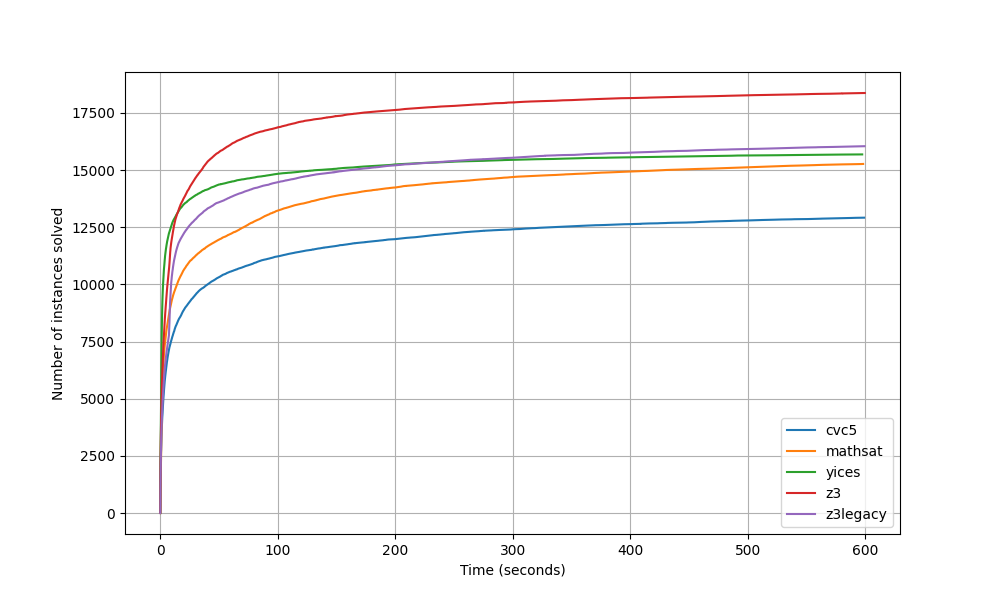
\includegraphics[width=0.99\textwidth]{../data/compare-qf-nia.png}
  \caption{Compare solvers on QF-NIA }
  \label{fig:compare-qf-nia}
\end{figure}

\begin{table}
  \begin{tabular}{|l|c|c|c|c|c|c|c|}
    \hline
    Solver & $<$ 1s & 1 to 10s & 10 to 100s & 100 to 600s & $>$ 600s & unknown/unhandled & solved \\
    \hline
    CVC5 & 1540 & 1071 & 529 & 416 & 3391 & 0/0 & 3556 \\
    \hline
    MathSat5 & 2995 & 1065 & 1124 & 1184 & 577 & 0/2 & 6368 \\
    \hline
    Yices2 & 3638 & 2001 & 276 & 120 & 909 & 0/3 & 6035 \\
    \hline
    z3 & 2840 & 1161 & 1521 & 754 & 669 & 0/2 & 6276 \\
    \hline
    z3legacy & 2714 & 1059 & 1619 & 702 & 851 & 0/2 & 6094 \\
    \hline
    \end{tabular}
  \caption{Comparison among solvers on QF\_LIA \label{tab:compare-qf-lia}}
\end{table}
\begin{figure}[htbp]
  \centering
  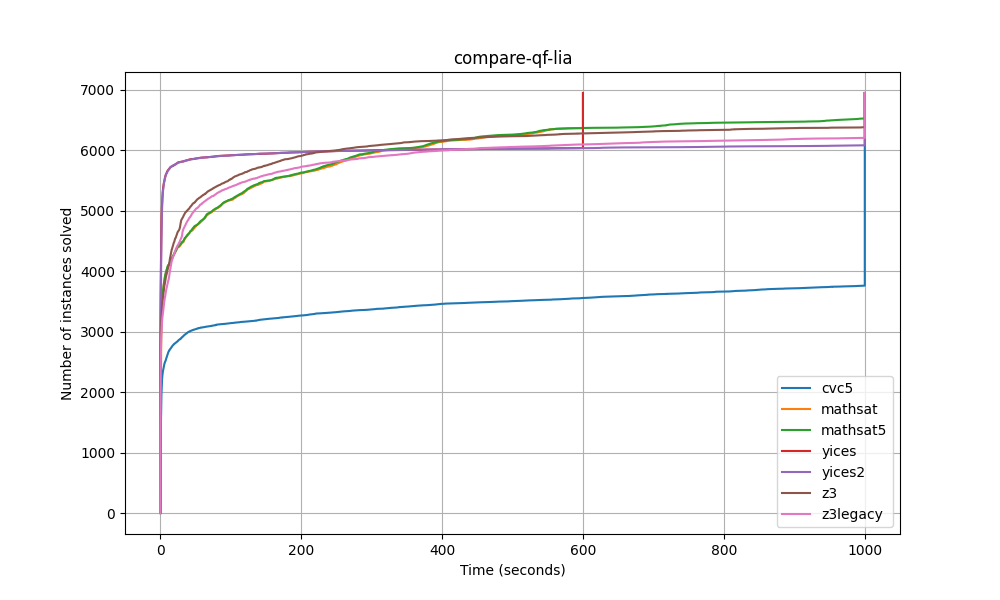
\includegraphics[width=0.99\textwidth]{../data/compare-qf-lia.png}
  \caption{Compare solvers on QF-LIA }
  \label{fig:compare-qf-lia}
\end{figure}


\begin{table}
  \begin{tabular}{|l|c|c|c|c|c|c|c|}
    \hline
    Solver & $<$ 1s & 1 to 10s & 10 to 100s & 100 to 600s & $>$ 600s & unknown/unhandled & solved \\
    \hline
    CVC5 & 11 & 23 & 54 & 33 & 183 & 4/0 & 121 \\
    \hline
    MathSat5 & 147 & 17 & 19 & 32 & 70 & 0/23 & 215 \\
    \hline
    Yices2 & 13 & 21 & 16 & 12 & 90 & 0/156 & 62 \\
    \hline
    z3 & 26 & 88 & 86 & 17 & 91 & 0/0 & 217 \\
    \hline
    z3legacy & 36 & 69 & 55 & 8 & 133 & 7/0 & 168 \\
    \hline
    \end{tabular}
  \caption{Comparison among solvers on Certora Benchmarks \label{tab:compare-benchmark-submission}}
\end{table}
\begin{figure}[htbp]
  \centering
  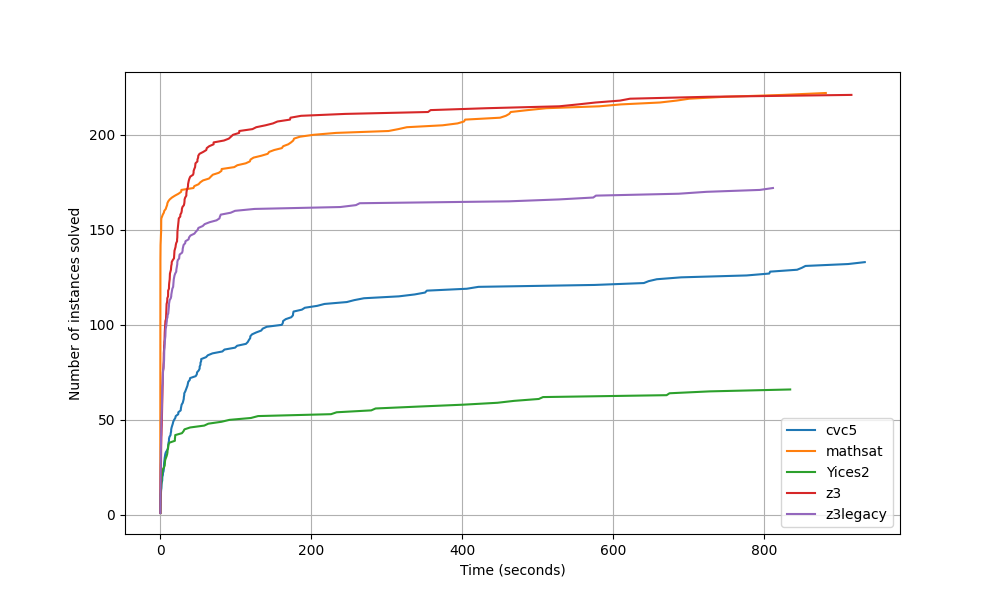
\includegraphics[width=0.99\textwidth]{../data/compare-benchmark-submission.png}
  \caption{Compare solvers on Certora Benchmarks
  \label{fig:compare-benchmark-submission}}
\end{figure}

\papercomment{
\begin{table}
  \begin{tabular}{|l|c|c|c|c|c|c|c|}
    \hline
    Disabled feature & $<$ 1s & 1 to 10s & 10 to 100s & 100 to 600s & $>$ 600s & unknown/unhandled & solved \\
    \hline
    gomory-use-big-cuts & 31 & 82 & 74 & 17 & 104 & 0/0 & 204 \\
    \hline
    bounded-nra & 30 & 83 & 81 & 18 & 96 & 0/0 & 212 \\
    \hline
    branching & 31 & 84 & 85 & 14 & 94 & 0/0 & 214 \\
    \hline
    gomory-use-closest-int & 31 & 83 & 85 & 16 & 93 & 0/0 & 215 \\
    \hline
    divisions-check & 29 & 92 & 77 & 19 & 91 & 0/0 & 217 \\
    \hline
    enable-gcd & 29 & 86 & 89 & 17 & 87 & 0/0 & 221 \\
    \hline
    gomory-polarity & 27 & 86 & 78 & 18 & 99 & 0/0 & 209 \\
    \hline
    gomory-use-big-cuts & 29 & 83 & 75 & 17 & 104 & 0/0 & 204 \\
    \hline
    gomory-use-closest-int & 29 & 86 & 84 & 15 & 94 & 0/0 & 214 \\
    \hline
    factorization & 29 & 86 & 85 & 18 & 90 & 0/0 & 218 \\
    \hline
    propagate-eqs & 28 & 90 & 81 & 20 & 89 & 0/0 & 219 \\
    \hline
    propagate-linear & 28 & 89 & 80 & 19 & 92 & 0/0 & 216 \\
    \hline
    grobner & 29 & 85 & 82 & 18 & 94 & 0/0 & 214 \\
    \hline
    horner & 29 & 85 & 81 & 18 & 95 & 0/0 & 213 \\
    \hline
    incremental-linearization & 30 & 73 & 70 & 10 & 125 & 0/0 & 183 \\
    \hline
    monic-eq & 28 & 89 & 83 & 18 & 90 & 0/0 & 218 \\
    \hline
    patch-monomials & 28 & 84 & 77 & 18 & 101 & 0/0 & 207 \\
    \hline
    gomory-polarity & 28 & 87 & 76 & 19 & 98 & 0/0 & 210 \\
    \hline
    propagate-monomial-bounds & 30 & 87 & 82 & 15 & 94 & 0/0 & 214 \\
    \hline
    \end{tabular}
  \caption{Disabling selected features on Certora Benchmarks \label{tab:benchmark-submission}}
\end{table}


\begin{table}
  \begin{tabular}{|l|c|c|c|c|c|c|c|}
    \hline
    Disabled feature & $<$ 1s & 1 to 10s & 10 to 100s & 100 to 600s & $>$ 600s & unknown/unhandled & solved \\
    \hline
    bounded-nra & 507 & 670 & 453 & 128 & 554 & 0/1 & 1758 \\
    \hline
    branching & 456 & 730 & 445 & 138 & 544 & 0/0 & 1769 \\
    \hline
    divisions-check & 462 & 701 & 470 & 138 & 541 & 0/1 & 1771 \\
    \hline
    enable-gcd & 461 & 716 & 449 & 137 & 549 & 0/1 & 1763 \\
    \hline
    gomory-use-big-cuts & 457 & 712 & 466 & 130 & 547 & 0/1 & 1765 \\
    \hline
    gomory-polarity & 452 & 724 & 460 & 135 & 542 & 0/0 & 1771 \\
    \hline
    gomory-use-closest-int & 456 & 709 & 468 & 139 & 541 & 0/0 & 1772 \\
    \hline
    grobner & 467 & 738 & 440 & 117 & 551 & 0/0 & 1762 \\
    \hline
    horner & 457 & 721 & 468 & 126 & 541 & 0/0 & 1772 \\
    \hline
    incremental-linearization & 402 & 498 & 286 & 106 & 1015 & 0/6 & 1292 \\
    \hline
    patch-monomials & 424 & 684 & 491 & 152 & 562 & 0/0 & 1751 \\
    \hline
    propagate-monomial-bounds & 433 & 697 & 478 & 156 & 549 & 0/0 & 1764 \\
    \hline
    \end{tabular}
  \caption{Disabling selected features on a representative small subset of QF\_NIA \label{tab:qf-nia-small}}
\end{table}


\begin{table}
  \begin{tabular}{|l|c|c|c|c|c|c|c|}
    \hline
    Disabled feature & $<$ 1s & 1 to 10s & 10 to 100s & 100 to 600s & $>$ 600s & unknown/unhandled & solved \\
    \hline
    enable-gcd & 2817 & 1151 & 1517 & 776 & 684 & 0/2 & 6261 \\
    \hline
    gomory-use-big-cuts & 2805 & 1164 & 1525 & 773 & 678 & 0/2 & 6267 \\
    \hline
    gomory-use-closest-int & 2815 & 1170 & 1528 & 758 & 674 & 0/2 & 6271 \\
    \hline
    gomory-polarity & 2850 & 1135 & 1525 & 750 & 685 & 0/2 & 6260 \\
    \hline
    \end{tabular}
  \caption{Comparison of selected integer linear arithmetic features on QF\_LIA \label{tab:qf-lia}}
\end{table}

}

%\section{Evaluation Data}
\label{app:eval}

We compare how many instances the solvers handle within
1s, within 1-10s, 10-100s, and 10-600s. We also list
timeouts and cases where the solver returns unknown because of incompleteness,
and cases where benchmarks are unhandled, either because the solver runs out of allocated virtual memory set to 2GB,
or due to unsupported features. The version of Z3 used for the experiments correponds to 4.12.5.


\begin{table}
  \begin{tabular}{|l|c|c|c|c|c|c|c|}
    \hline
    Solver & $<$ 1s & 1 to 10s & 10 to 100s & 100 to 600s & $>$ 600s & unknown/unhandled & solved \\
    \hline
    CVC5 & 3082 & 4564 & 3578 & 1693 & 10959 & 0/0 & 12917 \\
    \hline
    MathSat5 & 3304 & 6022 & 3894 & 2047 & 8607 & 0/2 & 15267 \\
    \hline
    Yices2 & 6372 & 6284 & 2176 & 852 & 8192 & 0/0 & 15684 \\
    \hline
    z3 & 4597 & 7440 & 4826 & 1504 & 5505 & 0/4 & 18367 \\
    \hline
    z3legacy & 3504 & 6881 & 4081 & 1577 & 6923 & 891/19 & 16043 \\
    \hline
    \end{tabular}
  \caption{Comparison among solvers on QF\_NIA \label{tab:compare-qf-nia}}
\end{table}


\begin{table}
  \begin{tabular}{|l|c|c|c|c|c|c|c|}
    \hline
    Solver & $<$ 1s & 1 to 10s & 10 to 100s & 100 to 600s & $>$ 600s & unknown/unhandled & solved \\
    \hline
    CVC5 & 1540 & 1071 & 529 & 416 & 3391 & 0/0 & 3556 \\
    \hline
    MathSat5 & 2995 & 1065 & 1124 & 1184 & 577 & 0/2 & 6368 \\
    \hline
    Yices2 & 3638 & 2001 & 276 & 120 & 909 & 0/3 & 6035 \\
    \hline
    z3 & 2840 & 1161 & 1521 & 754 & 669 & 0/2 & 6276 \\
    \hline
    z3legacy & 2714 & 1059 & 1619 & 702 & 851 & 0/2 & 6094 \\
    \hline
    \end{tabular}
  \caption{Comparison among solvers on QF\_LIA \label{tab:compare-qf-lia}}
\end{table}



\begin{table}
  \begin{tabular}{|l|c|c|c|c|c|c|c|}
    \hline
    Solver & $<$ 1s & 1 to 10s & 10 to 100s & 100 to 600s & $>$ 600s & unknown/unhandled & solved \\
    \hline
    CVC5 & 11 & 23 & 54 & 33 & 183 & 4/0 & 121 \\
    \hline
    MathSat5 & 147 & 17 & 19 & 32 & 70 & 0/23 & 215 \\
    \hline
    Yices2 & 13 & 21 & 16 & 12 & 90 & 0/156 & 62 \\
    \hline
    z3 & 26 & 88 & 86 & 17 & 91 & 0/0 & 217 \\
    \hline
    z3legacy & 36 & 69 & 55 & 8 & 133 & 7/0 & 168 \\
    \hline
    \end{tabular}
  \caption{Comparison among solvers on Certora Benchmarks \label{tab:compare-benchmark-submission}}
\end{table}


\begin{table}
  \begin{tabular}{|l|c|c|c|c|c|c|c|}
    \hline
    Disabled feature & $<$ 1s & 1 to 10s & 10 to 100s & 100 to 600s & $>$ 600s & unknown/unhandled & solved \\
    \hline
    gomory-use-big-cuts & 31 & 82 & 74 & 17 & 104 & 0/0 & 204 \\
    \hline
    bounded-nra & 30 & 83 & 81 & 18 & 96 & 0/0 & 212 \\
    \hline
    branching & 31 & 84 & 85 & 14 & 94 & 0/0 & 214 \\
    \hline
    gomory-use-closest-int & 31 & 83 & 85 & 16 & 93 & 0/0 & 215 \\
    \hline
    divisions-check & 29 & 92 & 77 & 19 & 91 & 0/0 & 217 \\
    \hline
    enable-gcd & 29 & 86 & 89 & 17 & 87 & 0/0 & 221 \\
    \hline
    gomory-polarity & 27 & 86 & 78 & 18 & 99 & 0/0 & 209 \\
    \hline
    gomory-use-big-cuts & 29 & 83 & 75 & 17 & 104 & 0/0 & 204 \\
    \hline
    gomory-use-closest-int & 29 & 86 & 84 & 15 & 94 & 0/0 & 214 \\
    \hline
    factorization & 29 & 86 & 85 & 18 & 90 & 0/0 & 218 \\
    \hline
    propagate-eqs & 28 & 90 & 81 & 20 & 89 & 0/0 & 219 \\
    \hline
    propagate-linear & 28 & 89 & 80 & 19 & 92 & 0/0 & 216 \\
    \hline
    grobner & 29 & 85 & 82 & 18 & 94 & 0/0 & 214 \\
    \hline
    horner & 29 & 85 & 81 & 18 & 95 & 0/0 & 213 \\
    \hline
    incremental-linearization & 30 & 73 & 70 & 10 & 125 & 0/0 & 183 \\
    \hline
    monic-eq & 28 & 89 & 83 & 18 & 90 & 0/0 & 218 \\
    \hline
    patch-monomials & 28 & 84 & 77 & 18 & 101 & 0/0 & 207 \\
    \hline
    gomory-polarity & 28 & 87 & 76 & 19 & 98 & 0/0 & 210 \\
    \hline
    propagate-monomial-bounds & 30 & 87 & 82 & 15 & 94 & 0/0 & 214 \\
    \hline
    \end{tabular}
  \caption{Disabling selected features on Certora Benchmarks \label{tab:benchmark-submission}}
\end{table}


\begin{table}
  \begin{tabular}{|l|c|c|c|c|c|c|c|}
    \hline
    Disabled feature & $<$ 1s & 1 to 10s & 10 to 100s & 100 to 600s & $>$ 600s & unknown/unhandled & solved \\
    \hline
    bounded-nra & 507 & 670 & 453 & 128 & 554 & 0/1 & 1758 \\
    \hline
    branching & 456 & 730 & 445 & 138 & 544 & 0/0 & 1769 \\
    \hline
    divisions-check & 462 & 701 & 470 & 138 & 541 & 0/1 & 1771 \\
    \hline
    enable-gcd & 461 & 716 & 449 & 137 & 549 & 0/1 & 1763 \\
    \hline
    gomory-use-big-cuts & 457 & 712 & 466 & 130 & 547 & 0/1 & 1765 \\
    \hline
    gomory-polarity & 452 & 724 & 460 & 135 & 542 & 0/0 & 1771 \\
    \hline
    gomory-use-closest-int & 456 & 709 & 468 & 139 & 541 & 0/0 & 1772 \\
    \hline
    grobner & 467 & 738 & 440 & 117 & 551 & 0/0 & 1762 \\
    \hline
    horner & 457 & 721 & 468 & 126 & 541 & 0/0 & 1772 \\
    \hline
    incremental-linearization & 402 & 498 & 286 & 106 & 1015 & 0/6 & 1292 \\
    \hline
    patch-monomials & 424 & 684 & 491 & 152 & 562 & 0/0 & 1751 \\
    \hline
    propagate-monomial-bounds & 433 & 697 & 478 & 156 & 549 & 0/0 & 1764 \\
    \hline
    \end{tabular}
  \caption{Disabling selected features on a representative small subset of QF\_NIA \label{tab:qf-nia-small}}
\end{table}


\begin{table}
  \begin{tabular}{|l|c|c|c|c|c|c|c|}
    \hline
    Disabled feature & $<$ 1s & 1 to 10s & 10 to 100s & 100 to 600s & $>$ 600s & unknown/unhandled & solved \\
    \hline
    enable-gcd & 2817 & 1151 & 1517 & 776 & 684 & 0/2 & 6261 \\
    \hline
    gomory-use-big-cuts & 2805 & 1164 & 1525 & 773 & 678 & 0/2 & 6267 \\
    \hline
    gomory-use-closest-int & 2815 & 1170 & 1528 & 758 & 674 & 0/2 & 6271 \\
    \hline
    gomory-polarity & 2850 & 1135 & 1525 & 750 & 685 & 0/2 & 6260 \\
    \hline
    \end{tabular}
  \caption{Comparison of selected integer linear arithmetic features on QF\_LIA \label{tab:qf-lia}}
\end{table}



\section{Summary and Discussion}

We presented the architecture and a cross-cut of system innovations in a new arithmetic solver in Z3.
It is shown to provide good advances relative to the legacy arithmetic solver,
and our evaluation suggests it compares very well with other state-of-art SMT solvers.
The new solver enabled us to addresses some design choices with the previous solver that limited extensibility.
Notably, the new solver separates its representation of arithmetic constraints from terms shared by other solvers through an E-graph.
We noticed that limitation of using shared terms is that the boundary for when to treat a sub-term as a variable or a polynomial is inherently
ambiguous. The legacy solver is also highly incomplete for non-linear
reasoning (over the reals). 

Many avenues for further innovations and tuning remain. Another important aspect is trust.
Implementing the many features of the arithmetic solver is inherently a complex task.
Many bugs get uncovered by fuzzing~\cite{DBLP:conf/sat/BrummayerLB10,DBLP:conf/sigsoft/MansurCWZ20,winterer-zhang-su-oopsla2020,winterer-zhang-su-pldi2020,DBLP:journals/pacmpl/ParkWZS21,DHuang,Maolin23} both in the legacy and new solver, 
bearing witness to the difficulty of creating a correct solver. The solver therefore supports a number of ways to validate results.
The easiest validation is for satisfiable formulas, where the satisfiable formula is model checked against the returned model.
The main difficulty with satisfiable models is to correctly track interpretations of under-specified operations, such as division by 0.
To check that consequences produced by the solver are valid, there is a self-validator 
enabled by the {\tt smt.arith.validate=true}. It uses the legacy arithmetic solver
to check lemmas and propagations. 
There is also a mechanism for creating certificates that can be processed offline or online.
With each theory axiom and propagation produced by the solver, it produces a certificate object that can be used to validate
inferences by the arithmetic solver. The certificates are exposed in proof objects~\cite{MouraB08b} and also as annotations in proof logs~\cite{z3prooflogs}.
Z3 contains a built-in proof checker for proof logs. The proof checker for arithmetic certificates validates
conflicts that can be justified by using Farkas lemma and bounds propagations that use cuts. It currently falls back to invoking
Z3 on lemmas (using the legacy arithmetic solver) for non-linear lemmas and other cases not covered by the built-in checker.
Certificates created for {\tt QF\_LRA} are fully handled, while self-contained or independent proof checking for more expressive fragments
of arithmetic is future work.


\bibliographystyle{plain}
\bibliography{refs}

%\appendix
%\section{Integers}
\label{app:ip}

\subsection{Patching}
\label{app:ip-patching}

We here outline the method for patching in more detail.

Given a row $x_b + \alpha y + r = 0$, where
$x_b$ is a basic variable, $y$ is non-basic variable multiplied by the fraction $\alpha$,
and $r$ is the remainding of the row, the shift amount $\delta$ is computed based on the
following analysis.

Take first the fractional parts of $\eval{x_b}$ and $\alpha$:

\begin{itemize}
\item $f_x := x_1/x_2 := \mathrm{frac}(\eval{x_b})$, s.t. $0 < x_1 < x_2$, and $x_1, x_2$ are mutually prime.
\item $f_\alpha := a_1/a_2 := \mathrm{frac}(\alpha)$, s.t. $0 < a_1 < a_2$, and $ a_1, a_2 $ are mutually prime.
\end{itemize}

The goal is to compute integers

\begin{itemize}
\item $\min \delta^+ > 0 \ . \ \mathrm{frac}(\alpha\delta^+) = 1 - f_x$,
\item $\max \delta^- < 0 \ . \ \mathrm{frac}(\alpha\delta^-) = 1 - f_x$.
\end{itemize}
These two integers are the minimal amount to move the value $\eval{y}$ to make the value of $\eval{x_b}$ integral.

Let $\Int$ be the set of integers.
We solve for $\delta \in \Int$ such that $L := \frac{x_1}{x_2}+\frac{a_1}{a_2}\delta \in \Int$ too. 
If $L \in \Int$ then $a_2 \frac{x_1}{x_2}+ a_1\delta$ is also an integer. Therefore $a_2 \frac{x_1}{x_2} \in \Int$. 
That means $a_2 := t x_2$ for some $t \in \Int$, because $x_1$ and $x_2$ are coprime. 
By substituting $a_2$ with $x_2 t$ we get $L:= \frac{x_1}{x_2}+\frac{a_1}{x_2 t}\delta$ and $L x_2 := x_1+\frac{a_1}{t}\delta \in \Int$.
Since $t \uparrow a_2$, and $a_2$ and $a_1$ are coprime, $t \uparrow \delta$. Therefore, we search for $\delta$ in form $\delta :=m t$, $m \in \Int$.
 We obtain $L:=  \frac{x_1}{x_2}+\frac{a_1}{x_2 t} m t = \frac{x_1+m a_1}{x_2}$. 
 From $L \in \Int$ follows $x_2 k = x_1 + m a_1$ for some $k \in \Int$. We can rewrite the 
 last equality as $x_1 =  a_1 m - x_2 k$. Because $x_2 \uparrow a_2$, and $a_1$ and $a_2$ are coprime, $x_2$ and $a_1$ are mutually prime too. That means that for some $u, v$ we have 
 $1 = a_1 u + x_2 v$. We can show that if $\delta := u t x_1$ then $\frac{x_1}{x_2}+\frac{a_1}{a_2}\delta \in \Int$. 
 

From the other side, for any $\gamma \in \Int$ satisfying $\frac{x_1}{x_2}+\frac{a_1}{a_2}\gamma \in \Int$
holds $\frac{a_1(\delta - \gamma)}{a_2} \in \Int$. 
Since $a_1$ and $a_2$ are coprime, $a_2 \uparrow (\delta - \gamma)$, and $\gamma := \delta \mod a_2$. We conclude that $\delta^+ = \delta \mod a_2$, and $\delta^{-} = \delta^+ - a_2$.

\subsection{Row Integral Variables}
\label{app:row-integral}

To show our reasoning we represent the set of non-basic row indices as the union of two disjoint subsets $A \cup B$, where $\{x_j:j \in A\}$ is the set of all row integral variables and $B$ is the rest of non-basic indices.
The row then can be written as $\sum_{j \in A} a_j\cdot x_j + \sum_{j \in B} a_j\cdot x_j + x_b = 0$, that is equivalent to $\sum_{j \in A} a_j\cdot x_j + x_b = -\sum_{j \in B} a_j\cdot x_j$. 

By choice of $A$ and the fact that $x_b$ is integral, the left-hand side has to be integral, but currently the fractional part of the left side value is equal to $\eval{x_b} - \lfloor \eval{x_b} \rfloor$, called $f_0$ in~\cite{DutertreM06}. Further on we can repeat all the steps of the proof of the Gomory inequality from~\cite{DutertreM06}, starting from the observation that the right-hand side value change should be either greater than or equal to $1 - f_0$, or smaller than or equal to $-f_0$, for the left-hand side to become integral.



\end{document}










